\selectlanguage{german}
%-----------------------------------------------------------------------------
\chapter{Umsetzung}\label{chap:Umsetzung}
%-----------------------------------------------------------------------------
\chapterstart
In diesem Kapitel wird die Umsetzung der Anforderungen in die Software erläutert. Es werden dabei besonders die Aspekte der Datenpersistenz, der Concurrency und der Skalierbarkeit vorgestellt.
\section{Überblick und Architektur}
Ausgehend von den Anforderungen wurde die Umsetzung des Schedulers\footnote{Die Umsetzung erfolgte unter dem Namen \textit{dJob}.} in Verantwortlichkeiten geteilt:
\begin{enumerate}
	\item Die Start-Prozedur
	\item Die \textit{Worker} die die Umsetzung der Aufgaben übernehmen
	\item Das Ausführen der Aufgaben \textit{Job} und planen der nächsten Ausführungszeit - der \textit{Scheduler}
	\item Das Laden von Aufgaben - der \textit{JobLoader}
\end{enumerate}
Die Trennung der Umsetzung erfolgte für den Scheduler und den JobLoader durch Interfaces gekapselt (siehe \ref{fig:architecture}). Die Instanziierung der tatsächlichen Klassen erfolgt zur Laufzeit über \textit{dependency injection}\cite{fowler2004}. Damit können diese Teile ausgetauscht werden und in etwa der Scheduler durch einen Echtzeit-fähigen Scheduler ausgetauscht werden ohne am Code selbst etwas ändern zu müssen\footnote{Die Umsetzung der injection dependency erfolgt in der Klasse \textit{ObjectRepository} ebenso um Rahmen dieser Arbeit. Umgesetzt wurde eine von außen konfigurierbare, explizite injection, einem \textit{service locator} nach Fowler. Verwendet wird diese mittels \code{var service = ObjectRepository.Get<ServiceType().}}.
\begin{figure}
	\centering
	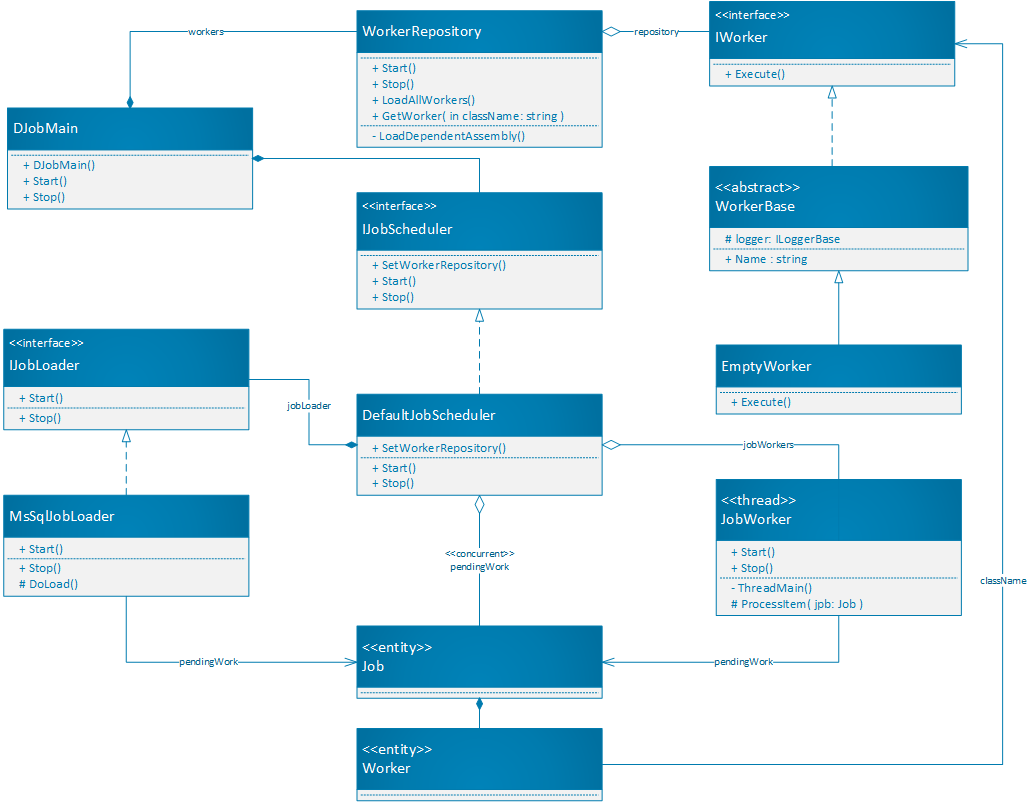
\includegraphics[width=0.7\linewidth]{images/architecture.png}
	\caption{Architekturübersicht des Schedulers, eigene Darstellung}
	\label{fig:architecture}
\end{figure}
Nach dem Start und der Initialisierung werden die Tasks die als nächstes ausgeführt werden sollen durch den JobLoader geladen und für andere Instanzen gesperrt. Dies geschieht durch das setzen des aktuellen Servers im Job (\code{Job.AllocatedTo}). Damit werden diese Jobs von anderen Instanzen ignoriert. Die Jobs werden dann in die interne Warteschlange (\code{pendingWork}) eingetragen.
\\Die Jobs in der Warteschlange werden durch die einzelnen Threads abgeholt, verarbeitet und die Job-Daten inklusiver dem Zeitpunkt der nächsten Ausführung in der Datenbank aktualisiert.
\\Die Verarbeitung selbst wird durch die Implementation des \code{IWorker} der für den Job vorgesehen ist (\code{Job.Worker}) erledigt. Welche Arbeiten verrichtet werden ist dem System nicht bekannt. Diese Worker werden durch den Klassennamen identifiziert und beim Starten des Systems aus dynamischen Bibliotheken geladen und instantiiert (siehe Kapitel \ref{sec:dynload}). Diese Entkopplung entspricht dem \emph{Command Pattern} \parencite{gamma1995}. Der \code{JobWorker} nimmt die Rolle des Receivers und des Clients gleichzeitig ein, da er vor der Ausführung noch das gewünschte ConcreteCommand aussucht.

\section{Datenbank}
Die Datenbank dient zur Speicherung aller notwendigen Daten. Es werden - ausgenommen Ablaufprotokolle - keine Daten anderswo gespeichert. Damit sind die Informationen zu den Jobs und zu deren Ausführungen zentral für alle Benutzer einsehbar und es können auch die Zugriffsrechte für Benutzer an einer Stelle gesteuert werden. Weiters werden Techniken die die Datenbank bereitstellt genutzt um eine Skalierung zu unterstützen (siehe Kapitel \ref{sec:scaling}).
\subsection{Datenbankmodell}
Das Datenbankmodell ist simpel gehalten und entspricht der \emph{dritten Normalform}. Es gibt also (vgl. \parencite[S. 317ff]{dbgrund})\begin{itemize}
	\item keine Felder die mehrere Werte enthalten (erste Normalform),
	\item keine Felder die die selbe Art von Werten enthalten (zweite Normalform)\footnote{Also in etwa die Felder Ausführungszeitpunkt1, Ausführungszeitpunkt2 ...}
	\item keine Wiederholungen von nicht-Schlüsselwerten in mehreren Datensätzen (dritte Normalform)
\end{itemize}
\begin{figure}
	\centering
	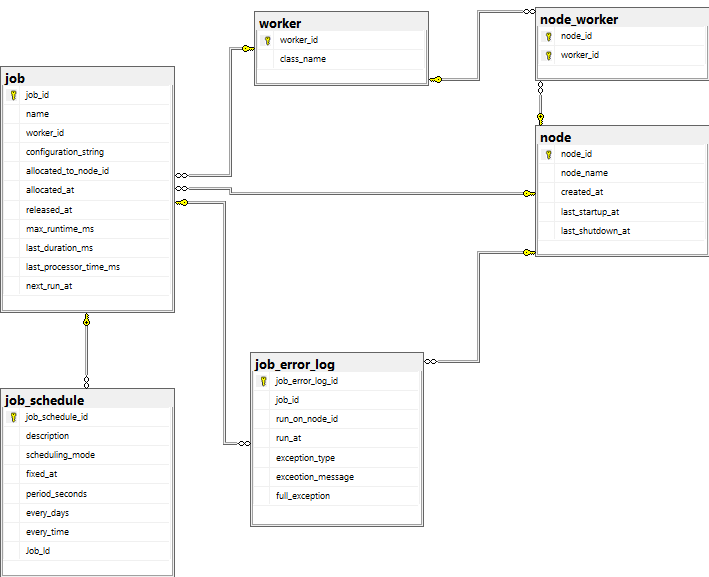
\includegraphics[width=0.7\linewidth]{images/dbmodel.png}
	\caption{Datenbankmodell, eigene Darstellung}
	\label{fig:dbmodel}
\end{figure}
Folgende Entitäten finden sich im Datenmodell:
\begin{itemize}
	\item worker - Enthält den Klassennamen der Instanz die die Abarbeitung der Arbeit der jobs übernehmen.
	\item node - Enthält einen Eintrag für jeden Server der eine Instanz von dJob ausführt.
	\item node\_worker - Ist eine \emph{intersection table}\footnote{Mithilfe einer intersection table wird eine m:n Beziehung zwischen Entitäten dargestellt.\parencite{oracle_intersection}} die die in einer Instanz verfügbaren Worker enthält.
	\item job - Enthält die Jobs die auszuführen sind. 
	\item job\_schedule - Enthält zu jedem Job ein oder mehrere Ausführungszeitpunkte oder einen Hinweis wie der job zu verplanen ist (\code{scheduling\_mode}).
	\item job\_error\_log - Enthält Details zu Fehlern (Exceptions) die während der Ausführung aufgetreten sind. Damit kann der Administrator den Grund für den Fehler feststellen.\footnote{Hier wurde das Protokollieren in die Datenbank gewählt da dies im Gegensatz zu einer Protokolldatei leichter in einer verteilten Umgebung zugänglich ist.}
\end{itemize}
Die Primärschlüssel in den Tabellen wurden als \emph{Unique Identifier} umgesetzt. Dies ist eine Zeichenfolge die errechnet werden kann. Diese hat den Vorteil gegenüber einer numerischen \emph{Identity}, also einem eindeutigen, monoton steigendem Wert der beim Einfügen in die Datenbank durch diese vergeben wird, dass im Falle von verteilten Systemen die Erstellung der Id weniger aufwendig ist, da diese ohne Synchronisierung auf der verteilten Datenbankinstanzen errechnet werden kann. Bei der Verwendung von Identities müssen die Werte, da sie ja eindeutig sein müssen, zwischen den Instanzen synchronisiert werden, was einen Mehraufwand bedeutet. 
\\Der Nachteil der sich unter Umständen aus der Verschlechterung des Index aus der stärkeren Streuung der Werte gibt, wird in diesem Fall in Kauf genommen da in der Regel für den Zugriff andere Indices verwendet werden.\parencite{ms_guid}
\subsection{Zugriff}
Der Zugriff auf die Datenbank erfolgt mittels dem Microsoft Entity Framework (im folgenden kurz EF) in der Version 6. Dies ist eine \emph{ORM (Object Relational Mapping)} Bibliothek die die Datenbank hinter einer Zugriffsschicht verbirgt und die relationalen Daten (Datensätze) direkt in Objekte umwandelt. Damit ist für den Entwickler kein Bruch zwischen Datenbank und objektorientierter Anwendungsentwicklung erkennbar.
\\Dieser Ansatz wird in der Umsetzung vollständig verfolgt in dem die so genannte \emph{code-first} Methode verwendet wird. Dabei
werden die Entitäten als C\# Klassen definiert und automatisch durch das EF die Datenbank erzeugt. 
\begin{lstlisting}[caption={Klassendefinition für Code-First, siehe Job.cs}, label={lst:codefirst}, captionpos=b]
    [Table("job")]
	public class Job
	{
		[Key]
		[Column("job_id")]
		[DatabaseGenerated( DatabaseGeneratedOption.Identity )]
		public Guid Id { get; protected set; }

		[Required]
		[MinLength(8)]
		[MaxLength(64)]
		[Column("name")]
		public string Name { get; protected set; }

		[Required]
		[Column("worker_id")]
		public Guid WorkerRef { get; protected set; }

		[ForeignKey("WorkerRef")]
		public virtual Worker Worker { get; set; }

		[Column("configuration_string")]
		public string ConfigurationString { get; set; }

		[Column("allocated_to_node_id")]
		public Guid? AllocatedToRef { get; protected set; }

		[ForeignKey(nameof( AllocatedToRef ) )]
		public virtual Node AllocatedTo { get; protected set; }

		[Column("allocated_at")]
		public DateTime? AllocatedAt { get; protected set; }

		[Column( "released_at" )]
		public DateTime? ReleasedAt { get; protected set; }
		
		// lines ommited
		
		public virtual ICollection<JobSchedule> Schedule { get; protected set; }
		
		//lines omitted
}
\end{lstlisting}
Über \emph{Annotierungen} können Eigenschaften in der Umsetzung geändert werden (siehe \parencite{eftut}). Mit den Annotierungen \code{Table} und \code{Column} können die Namen der Tabellen und Felder geändert werden. Für die Eigenschaft \code{Id}  werden zusätzlich die Annotierungen \code{Key} um diese als Primärschlüssel zu kennzeichnen, und \code{DatabaseGenerated} verwendet. Damit wird - da es sich um einen Unique Identifier handelt - ein default-Wert für die Spalte von \code{newsequentialid()} erzeugt. Die Datenbank generiert somit den Primärschlüssel selbst. \code{Required} definiert für die Eigenschaft \code{Name} eine not-null Beschränkung, der Wert muss also im Datensatz vorhanden sein. Zusätzlich sind für diese Eigenschaften noch eine minimale und maximale Länge gesetzt. Dies ist bei String-Typen von Bedeutung, da sonst automatisch ein String mit maximaler Länge in der Datenbank angelegt wird, was negative Auswirkungen auf die Laufzeit haben kann. 
\\Von Bedeutung sind auch die \code{virtual} Modifikatoren. Diese weisen das EF an, die Inhalte der Eigenschaften erst beim tatsächlichen Zugriff auf diese zu laden. Dies wird als \emph{lazy loading} bezeichnet. Damit werden Daten aus verbundenen Tabellen nur dann geladen, wenn diese benötigt wird. Ohne das lazy loading würden die Daten immer geladen werden, auch wenn diese gar nicht benötigt werden. Durch die Nutzung dieser Methode kann das verhalten zur Laufzeit verbessert werden da keine unnötigen Daten in der Datenbank gelesen werden. Die technische Umsetzung in EF erfolgt mittels des so genannten \emph{Proxy-Patterns} \footnote{ siehe \parencite[S. 207ff]{gamma1995}}\parencite{ms_proxy}. Dabei wird dynamisch durch das EF eine Instanz einer Klasse erzeugt die von der Entität erbt. Um das lazy loading zu Implementieren, werden in den Zugriffsfunktionen der Proxy-Klasse zuerst die Daten von der Datenbank geladen und erst danach an den Aufrufer zurückgegeben.
\\Der Zugriff auf die Daten erfolgt über einen so genannten \code{Context} der die notwendigen Operationen durchführt und die geladenen Objekte gegebenenfalls anreichert. Der Context speichert auch alle geladenen Objekte und erkennt und verfolgt Änderungen an den Objekten so dass alle Änderungen an geladenen Objekten über den Context mit einem einzigen Befehl (\code{Context.SaveChanges()}) gespeichert werden können.
\\Geladen werden die Abfragen über die C\# Spracherweiterung \emph{LINQ}\footnote{Language INtegrated Query - siehe \url{https://docs.microsoft.com/en-us/dotnet/csharp/programming-guide/concepts/linq/}}. Diese datenbankunabhängige Abfragesprache wird durch das EF in SQL übersetzt. Daher wird LINQ auch für Abfragen in interne Collections wie Listen verwendet.
\begin{lstlisting}[caption={LINQ Abfrage - Lambda Syntax, siehe DefaultJobLoader.cs - DoLoad()},label={lst:linq_fluent},captionpos=b]
	var q = dbContext.Jobs.Include( "Worker" )
			.Where( j => myNextJobIds.Contains( j.Id ) )
			.OrderBy( j => j.NextRunAt )
			.AsNoTracking( )
			;

\end{lstlisting}
Wie in Listings \ref{lst:linq_fluent} und \ref{lst:linq_expression} dargestellt ist, verfügt LINQ über zwei unterschiedliche Formen. Die so genannte \emph{Lambda} Syntax, bei der die Syntax der C\# Sprache beibehalten wird und \emph{Lambdas} einsetzt um Operationen durchzuführen. Und die \emph{Query Expression} Syntax, bei der eine SQL ähnliche Abfrage direkt im Code geschrieben werden kann. Beide Varianten sind in etwa gleich mächtig\footnote{Einige Funktionen stehen nur in der Lambda Syntax zur Verfügung} und können auch abwechselnd verwendet werden.\footnote{Die Query Expression Syntax ist genau genommen nur eine Syntax Erweiterung und wird in eine Lambda Expression umgewandelt.\parencite{linq}}
\begin{lstlisting}[caption={LINQ Abfrage - Query Expression Syntax},label={lst:linq_expression},captionpos=b]
	var q = from job in dbContext.Jobs
			where myNextJobIds.Contains( job.Id ) )
			orderby job.NextRunAt
			select job
		;
\end{lstlisting}
Zeile 1 in Listing \ref{lst:linq_fluent} definiert die Tabelle aus der die Daten geladen werden sollen. Die Erweiterung \code{.Include("Worker")} weist das EF an, die Daten der Eigenschaft \code{Worker} aus der verbundenen Tabelle ebenso gleich zu laden. Dies nennt man \emph{eager loading}. Damit werden alle Daten in einer Abfrage geladen, was positive Auswirkungen auf die Laufzeit hat.\footnote{Die Eigenschaft \code{Worker} ist virtuell und wird daher erst beim Zugriff geladen. Da aber an dieser Stelle im Code die Daten der \code{Worker} Eigenschaft benötigt werden, wird hier ein eager-loading erzwungen um performanter zu sein.}
\subsubsection{Laden der Jobs}
Das Laden der Jobs die ausgeführt werden sollen ist eine der kritischsten Stellen. Die Jobs müssen so rasch wie möglich geladen werden, ohne aber dabei andere laufende Instanzen zu behindern. Dies wird Mithilfe der Nutzung von Isolation Levels und Sperren erreicht. Dies ist nur mithilfe eines SQL Statements möglich, EF bietet auf dieser Ebene keine Unterstützung an.
\begin{lstlisting}[caption={Jobs Laden, siehe DefaultJobLoader.cs - DoLoad()},label={lst:jobloader},captionpos=b]
string loadCommand = $@"SELECT TOP {gulpSize}
				job.job_id
				, job.name
				, node.node_name
				FROM job
				WITH (XLOCK, ROWLOCK, READCOMMITTED , READPAST)
					JOIN node_worker ON ( node_worker.worker_id = job.worker_id )
					JOIN node ON ( node.node_id = node_worker.node_id AND node.node_name = @NodeId)
				WHERE job.allocated_to_node_id IS NULL
					AND job.next_run_at < CURRENT_TIMESTAMP
				ORDER BY job.next_run_at ASC";
\end{lstlisting}
Mit dem Statement in Codebeispiel \ref{lst:jobloader} werden die Id's der nächsten Jobs gelesen die auszuführen sind. Mit dem \code{join} der node\_worker Tabelle werden dabei nur die jobs berücksichtigt, die in dieser Instanz ausgeführt werden können. Die Abfrage \code{allocated\_to IS NULL} schließt Jobs aus die bereits in anderen Instanzen geladen sind. 
\\Die sogenannten \emph{Hinweise (hints)} (siehe \parencite{ms_hints}) in Zeile 6 wird das verhalten bei Nebenläufigkeit gesteuert.
\begin{itemize}
	\item \code{READCOMMITED} - Setzt die Isolationsstufe für dieses Statement. Damit werden Änderungen von anderen committeten Transaktionen gelesen, auch wenn diese nach dem Start der eigenen Transaktion erst committed wurden.\footnote{Siehe Kapitel \ref{subs:isolation}.} Die Isolationsstufe wird hier erzwungen, damit READPAST immer fehlerfrei angewendet werden kann.
	\item \code{READPAST} - Damit werden von anderen Transaktionen gesperrte Datensätze ignoriert und die Datensätze nach dem gesperrten gelesen. Ansonsten würde die Transaktion warten bis die Sperre auf dem Datensatz aufgehoben ist.
	\item \code{ROWLOCK} - Setzt eine Sperre auf Datensatzebene auf die gelesenen Datensätze.
	\item \code{XLOCK} - Weist die Datenbank an ein Exklusive Sperre zu setzen. Damit kann der Datensatz von keiner anderen Transaktion gelesen werden.
\end{itemize}
Nachdem die Jobs geladen wurden, werden sie in der selben Transaktion durch das setzen des Feldes \code{allocated\_to} logisch gesperrt und von anderen Instanzen nicht mehr geladen. Diese Vorgehensweise stellt sicher dass die Jobs nur von einer Instanz gelesen werden, aber andere Instanzen weitere auszuführende Jobs lesen kann. Die Anzahl der Jobs die gelesen werden ist durch die \code{TOP} Klausel beschränkt die von Administrator konfiguriert werden kann.\footnote{Diese Art der Übergabe von Parametern ist prinzipiell ein Sicherheitsrisiko (\emph{SQL-Injection}). Da der Parameter ein Integer Wert ist und dies durch die Anwendung sichergestellt ist, ist das Statement trotzdem sicher.}
\\Um die Transaktion so klein wie möglich zu halten und somit die gesetzten Datenbanksperren so kurz wie möglich zu halten, endet die Transaktion nach dem setzen der Node. In einer zweiten Transaktion danach werden erst die vollständigen Daten der allokierten Jobs geladen.
\\Nachdem alle Jobs geladen wurden, werden diese dem Arbeitsvorrat hinzugefügt. Die Details dazu sind in den Kapiteln \ref{sec:producerconsumer} und \ref{sec:blockingq} beschrieben.
\section{Skalierung}
Einer der ausschlaggebenden Gründe für die Entwicklung war, dass bisherige Lösungen hinsichtlich der Leistung schlecht skalieren. Die einzige Möglichkeit ist meist, einen stärkeren Server zu nutzen. Deswegen ist die leichte Skalierung der Leistung eine grundlegende Anforderung an das System. Um bestimmte Aufgaben effizient abarbeiten zu können, kann es notwendig sein, eine darauf ausgelegt Hardware zu verwenden, um in etwa Berechnungen auf einer GPU durchzuführen. Dies wird mit der Möglichkeit der funktionalen Skalierung erreicht.
\subsection{Skalierung der Leistung} \label{sec:scaling}
Das umgesetzte System bietet zwei Möglichkeiten die Leistung zu skalieren. Die erste Möglichkeit ist die Skalierung der Leistung innerhalb eines Servers durch die Konfiguration der maximal gleichzeitig laufenden Threads pro Instanz. Damit kann die für dJob zur Verfügung stehende Leistung sowohl erhöht, als auch beschränkt werden um andere, am selben Server laufende Applikationen nicht zu beeinflussen.
\\Die zweite Möglichkeit ist die Nutzung von mehren Servern. Dies ist durch dJob durch Installation des Services und der benötigten Worker erledigt. Es sind keinerlei weitere Anpassungen oder Konfigurationen nötig um das System zum Laufen zu bringen. 
\\Für die Installation gibt es drei grundlegende Möglichkeiten (siehe auch Darstellung \ref{fig:performance_scaling}):
\begin{enumerate}
	\item Szenario 1 - Ein Server, Datenbank und Applikation ist am selben Server installiert. Damit können kleine Systeme mit geringen Leistungsanforderungen umgesetzt werden.
	\item Szenario 2 - Mehrere Server, auf einem Server ist die Datenbank und die Applikation installiert, auf den restlichen Servern ist nur die Applikation installiert. Damit können mittlere Systeme, oder Systeme mit spezialisierter Hardware umgesetzt werden.
	\item Szenario 3 - Mehrere Server auf denen die Applikation installiert ist und die auf eine verteilte Datenbank auf mehreren Servern zugreifen. Damit können größte und weltweit verteilte Systeme umgesetzt werden.
\end{enumerate}
Durch die Verwendung eines Datenbanksystems zur Speicherung der Jobs ist die Konfiguration des dJob Services in allen Szenarien gleich. Es muss lediglich der \emph{connection string} der die Verbindung zur Datenbank definiert korrekt konfiguriert werden. Für das System und für die einzelnen Instanz hat das gewählte Szenario kein Auswirkungen und ist für die Anwendung auch nicht merkbar. Die Probleme die durch die Gleichzeitigkeit entstehen sind in der Datenbank und durch die Umsetzung des Ladens der Jobs abgefangen. 
\\Im dritten Szenario liegt die Komplexität der Konfiguration außerhalb des Systems bei der verteilten Datenbank. Dies kann in SQL-Server mittels einer \emph{transactional replication} zwischen Servern.\parencite{ms_resolve} Damit werden alle Daten in den Datenbanken und alle Daten die zur Verwaltung nötig sind (wie in etwa Sperren) zwischen den einzelnen Servern automatisch aktualisiert. Aus Sicht der Applikation ändert sich nichts, da eine verteilte Datenbank sich gegenüber Anwendungen wie eine einzelne Instanz verhält. Eine Variante des dritten Szenarios ist die Verwendung einer Cloud-basierten Datenbank. Diese ist aus Sicht der Applikation ident mit Szenario 3. Um bei der Verwendung einer Cloud-Datenbank immer genügend Arbeitsvorrat in einer Instanz zur Verfügung zu haben, kann es notwendig sein eine höhere \code{gulpSize} und eine höhere \code{lowWaterMark}\footnote{Das ist die Anzahl an Jobs im Arbeitsvorrat die unterschritten sein muss bevor neue Jobs geladen werden.} zu konfigurieren. Damit kann eine längere Dauer des Ladens der Jobs abgefangen werden.
\\In der beispielhaften Verwendung wurde das Szenario 2 umgesetzt und erreicht die derzeit nötige Leistung mit 3 Servern mit je 8 Kernen die über Österreich verteilt genutzt werden.
\begin{figure}
	\centering
	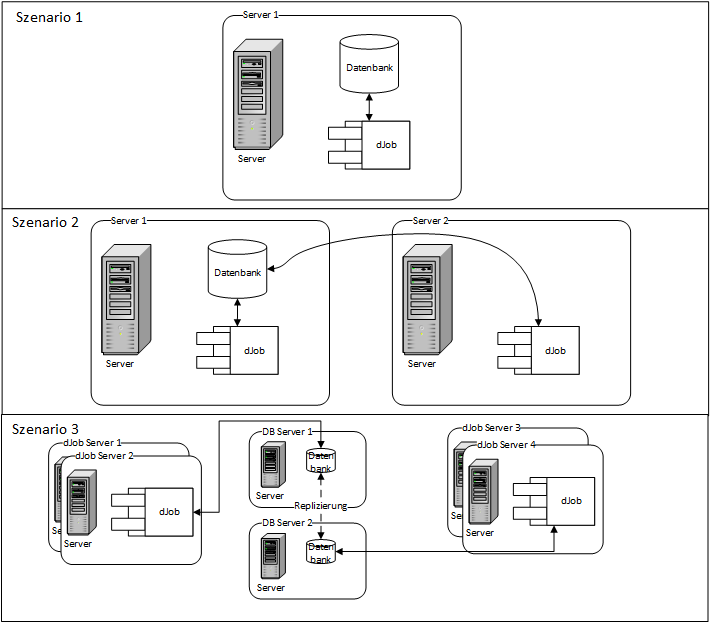
\includegraphics[width=0.7\linewidth]{images/scaling}
	\caption{Skalierung der Leistung, eigene Darstellung}
	\label{fig:performance_scaling}
\end{figure}

\subsection{Funktionale Skalierung} \label{sec:dynload}
Mithilfe der funktionalen Skalierungen werden zwei grundlegende Anforderungen erfüllt. Es können weitere Worker, also die Funktionen die die tatsächliche Arbeit verrichten, ohne Veränderung des dJob Systems umgesetzt werden, und die einzelnen dJob Instanzen können über unterschiedliche Worker besitzen um differenzierte Hardware der Server auszunutzen.
\\Um neue Worker zu definieren, müssen diese in einer \emph{\.NET Assembly} vorhanden sein. 
Diese ist die kleinste Einheit in der Code zur Verfügung gestellt werden kann. Sie enthält neben dem Programmcode\footnote{Dieser ist in der Assembly bereits in die \emph{Intermediate Language (IL)} kompiliert.} auch Metadaten, die unter anderem auch die Abhängigkeiten zu anderen Assemblies definieren. Eine Assembly wird typischerweise als eine Bibliothek (.dll) oder als direkt ausführbares Programm zur Verfügung (.exe) gestellt \parencite[S. 17ff]{box}. Das dJob Service wird als ausführbares Programm zur Verfügung gestellt, alle Assemblies von denen es abhängig ist, sind entweder .NET Standard-Assemblies oder, wie die dJob.core Bibliothek im selben Verzeichnis vorhanden und können somit durch .NET selbst geladen werden. Die Abhängigkeiten zu diesen Assemblies wird zum Zeitpunkt der Kompilierung ermittelt und in den Metadaten der .exe Datei gespeichert.
\\Um Programmcode zu nutzen der zum Zeitpunkt der Kompilierung nicht Teil von dJob war, müssen diese Assemblies zur Laufzeit \emph{dynamisch} geladen werden.Das dJob service sucht dazu in einem konfiguriertem Pfad alle Programmbibliotheken und lädt diese Assemblies in den Speicher, dies ist in Codebeispiel \ref{lst:dynamicloading} dargestellt. 
Worker - Klassen in den Bibliotheken die die Arbeit erledigen, müssen dabei \begin{enumerate}
	\item von außerhalb der Bibliothek sichtbar sein - nur so kann eine Klasse instanziiert werden
	\item vom Interface \code{at.loe.djob.core.worker.IWorker} erben
	\item einen parameterlosen Konstruktor haben.
\end{enumerate}
Alle im Verzeichnis vorhandenen Bibliotheken (Zeile 1) werden geladen (Zeile 3). Danach werden alle Klassen die das Interface \code{IWorker} implementieren (Zeile 5\&6) instantiiert (Zeile 8) und in einer Collection\footnote{Es handelt sich um ein \code{ConcurrentDictionary}. Dies ist eine Key/ Value Sammlung mit eindeutigen Keys die für die Verwendung durch mehrere Threads vorgesehen ist. Die Zugriffe auf die Collection sind immer thread-safe, alle eventuell notwendigen Sperren werden durch die Collection selbst verwaltet.} abgelegt (Zeile 12).
\begin{lstlisting}[caption={Dynamic Loading, siehe WorkerRepository.cs - LoadAllWorkers()},label={lst:dynamicloading},captionpos=b]
foreach ( string file in  workerDirectory.GetFiles( "*.dll" ) )
{
	Assembly assembly = Assembly.LoadFile( file );

	foreach ( Type typeToLoad in assembly.GetTypes()
					.Where( t => t.ImplementsInterface<IWorker>() ) )
	{
		IWorker w = (IWorker)Activator.CreateInstance( typeToLoad );

		w.Initialize( ObjectRepository.Get<IConfigurationProvider>( ), logger );

		if( ! repository.TryAdd( typeToLoad.FullName, w ) )
		{
			throw new InvalidOperationException
			( $"Could not add class '{typeToLoad.FullName}' to repository");
		}
	}
}
\end{lstlisting}
Wenn die Bibliotheken die geladen werden sollen Abhängigkeiten zu anderen, nicht-Standard, Bibliotheken haben, so werden diese nur automatisiert aufgelöst und geladen wenn diese entweder global verfügbar sind oder in Verzeichnis des Services zu finden sind \parencite[S. 42ff]{box}). Liegen diese im Verzeichnis in dem auch die Worker-Bibliothek abgelegt ist, so muss diese Auflösung durch die Anwendung selbst erfolgen. Dafür stellt .NET das Ereignis \code{AssemblyResolve} zur Verfügung. Die Anwendung kann dann die benötigten Bibliotheken selbst suchen und laden\footnote{Siehe WorkerRepository.cs Methode \code{LoadDependentAssembly()}} \footnote{Wird dies nicht durch die Anwendung erledigt, so erhält man eine \code{FileNotFoundException} mit dem Name der Bibliothek \emph{die den Verweis enthält}, und nicht, den Namen der Bibliothek die nicht aufgelöst werden kann. }.
\\Nachdem alle Worker geladen wurde, werden diese in der Datenbank für die aktuelle Instanz aktualisiert, so dass beim Laden der Jobs für die Instanz nur diese Jobs geladen werden die auch ausgeführt werden können. Dadurch können für jede Instanz unterschiedliche Worker konfiguriert werden, was die zweite Anforderung abdeckt.
\section{Concurrency}
Um die Leistung eines Servers ausnutzen zu können werden die geladenen Jobs durch mehrere Threads parallel abgearbeitet. Dazu werden durch den \code{DefaultJobScheduler} die konfigurierte Anzahl an Threads angelegt und gestartet. Diese beziehen ihre Arbeit aus einer globalen Datenstruktur die Jobs und führen dann die für die Jobs konfigurierten Worker aus. Diese Architektur entspricht dem \emph{Producer/ Consumer Pattern} \parencite[S. 163ff]{jthreads}. Der \code{DefaultJobLoader} entspricht dabei dem Producer, die einzelnen \code{JobWorker} dabei den Consumern. Ein entscheidendes Element dieses Patterns ist die Datenstruktur die für die Entkopplung sorgt. Durch den Zugriff mehrere Threads muss diese einerseits thread-safe sein, andererseits müssen die Operationen so effizient wie möglich sein. Daher werden diese zwei Element näher betrachtet.
\subsection{Producer-Consumer}\label{sec:producerconsumer}
Der Producer/ Consumer Pattern ist einer der häufigst verwendeten Pattern wenn es um Abarbeitung von Aufgaben durch mehrere Threads geht. Er besteht aus 
\begin{itemize}
	\item ein oder mehreren Producern die in eigenen Threads laufen und Arbeitspakete produzieren
	\item einer zentralen Datenstruktur, in die Producer die Arbeitspakete einfügen und die Consumer diese entfernen
	\item ein oder mehrere Consumer, die wiederum als eigene Threads laufen und die Arbeitspakete aus der zentralen Datenstruktur holen und abarbeiten.
\end{itemize}
Dies ist auch in Abbildung \ref{fig:architecture} dargestellt.\parencite{jthreads}
\begin{figure}
	\centering
	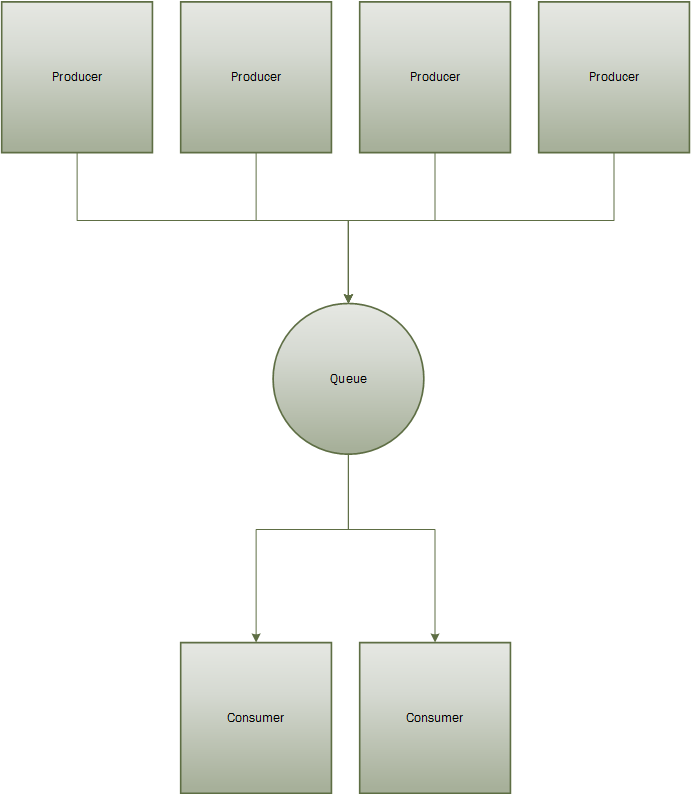
\includegraphics[width=0.7\linewidth]{images/B2_Producer_Consumer_1}
	\caption{Producer/ Consumer Darstellung, vgl. \parencite[S. 163]{jthreads}}
	\label{fig:architecture}
\end{figure}
\\Die Verbreitung dürfte in seiner Einfachheit begründet sein. Denn sowohl Producer als auch Consumer, die jeweils in verschiedenen Threads ihre Arbeit verrichten brauchen beim Zugriff auf die Daten keine weiteren Aktionen durchführen\footnote{Dies gilt für die zu bearbeitenden Daten, beim Zugriff auf andere, globale Daten sind diese sehr wohl Sperren zu setzen.} \parencite[S. 163ff]{jthreads}. Der Schutz der Daten des Arbeitspaketes erfolgt durch die Datenstruktur, in der Regel eine Queue. Diese setzt innerhalb der öffentlichen Methoden die Sperren wenn nötig. Diese übernimmt auch die Aufgabe des Aufweckens von Consumern wenn Arbeit anliegt.
\\Der Pattern ist auch sehr vielseitig. In einer weiteren gebräuchlichen Form (siehe Abbildung \ref{fig:architecture_2}) ist die Verwendung von mehreren Queues und einem Dispatcher. Dies kann einerseits bei einer sehr hohen Anzahl an Producern oder Consumern verwendet werden, da dadurch die Häufigkeit der Sperren, und damit die Wartezeit eines Threads gesenkt wird. Weiters kann auch die Anzahl an Consumern pro Queue unterschiedlich sein. Damit kann der Dispatcher wichtigere Arbeitsaufgaben in die Queue legen der mehr Consumer zugeteilt sind. Damit erfolgt eine schnellere Abarbeitung des Arbeitspaketes.
\begin{figure}
	\centering
	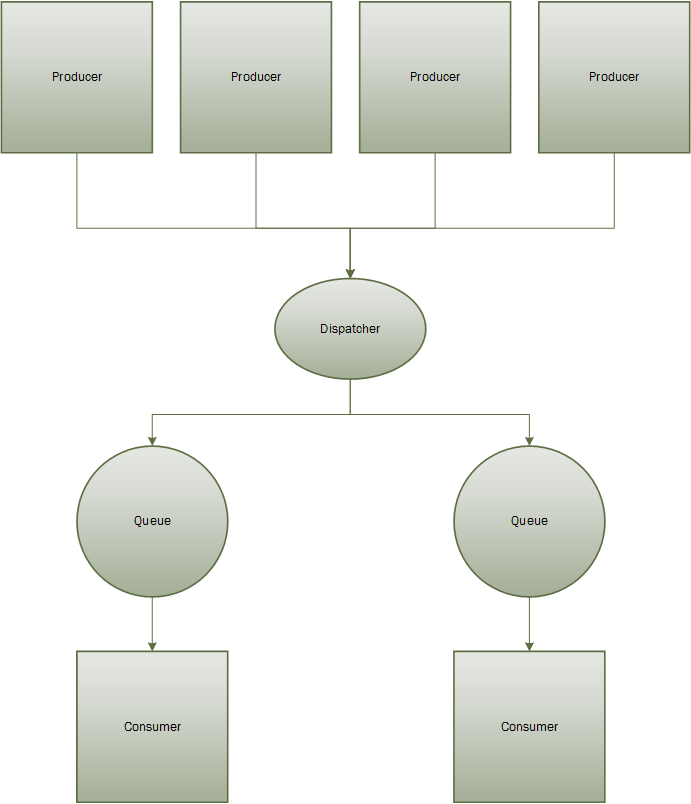
\includegraphics[width=0.7\linewidth]{images/pc_w_dispatcher}
	\caption{Producer/ Consumer Darstellung mit mehreren Queues, vgl. \parencite[S. 163]{jthreads}}
	\label{fig:architecture_2}
\end{figure}
\\Im dJob Service ist die Implementation des \code{IJobLoader} der einzelne Producer. Die vorab allokierten und gestarteten Instanzen der \code{JobWorker} bilden die Producer. Die zentrale Datenstruktur ist die \code{BlockingCollection} namens \code{pendingWork}.
\subsection{BlockingCollection}\label{sec:blockingq}
Wie im vorigen Kapitel beschrieben, leistet die zentrale Datenstruktur im Producer/ Consumer Pattern den Großteil der Arbeit was die Synchronisierung der einzelnen Threads betrifft. Daher ist das Design und die Implementierung dieser Klasse essentiell für die Leistung des Gesamtsystems. Die Klasse muss
\begin{itemize}
	\item sicherstellen dass die Methode zum Einfügen der Elemente thread-safe ist, also mehrere Threads zugleich Elemente einfügen können ohne die Datenstruktur zu beschädigen
	\item sicherstellen, dass die Methode zum Entfernen der Elemente thread-safe ist
	\item Consumer Threads suspendieren wenn keine weitere Arbeit anliegt
	\item Consumer Threads aufwecken wenn weitere Arbeit eingefügt wurde
	\item die Anzahl an gesetzten Sperren und die Zeitdauer der Sperre so gering wie möglich halten.
\end{itemize}
Codebeispiel \ref{lst:blockingQ} zeigt die Implementierung einer solchen Klasse. Zur Datenhaltung wird die Standardklasse \code{Queue} verwendet (\code{backingStore}), die selbst nicht thread-safe ist.
\begin{lstlisting}[caption={Implementierung BlockingQ, siehe MyBlockingQ.cs}, label={lst:blockingQ}, captionpos=b]
    public class MyBlockingQueue<T>
	{
		private Queue<T> backingStore = new Queue<T>();

		/// <summary>
		/// lock to protect the backingStore and used for notifications
		/// </summary>
		private readonly object myLock = new object();

		public MyBlockingQueue()
		{ /* empty */ }


		/// <summary>
		/// add an item to the queue in a threadsafe way
		/// </summary>
		public void Enque( T newElement )
		{
			lock( myLock )
			{
				backingStore.Enqueue( newElement );

				Monitor.Pulse( myLock );
			}
		}

		/// <summary>
		/// Take an item from the queue
		/// if no item is available, wait until an element has been put into the queue and check again
		/// </summary>
		/// <returns>an element from the q</returns>
		public T Dequeue( int millisecondsTimeout )
		{
			lock( myLock )
			{

				while ( ! backingStore.Any() )
				{
					if( !Monitor.Wait( myLock, millisecondsTimeout ) )
					{
						return default( T );
					}
				}

				return backingStore.Dequeue();
			}
		}
}
\end{lstlisting}
Die gezeigte Implementierung erfüllt alle genannten Bedingungen. In der Methode \code{Enque} wird innerhalb einer gesetzten Sperre ein Element der Sammlung hinzugefügt(Zeile 21). Und danach mittels eines Monitors ein suspendierter Consumer geweckt (Zeile 23)\footnote{Sollte kein Consumer suspendiert sein, so erfolgt keine Aktion.}. 
Die Consumer rufen die Methode \code{Deque} auf und erhalten entweder eine Element oder werden suspendiert. In der Methode wird eine Sperre gesetzt (Zeile 34) und danach geprüft ob Elemente vorhanden sind (Zeile 37). Wenn Elemente vorhanden sind, wird das erste Element der Queue zurückgegeben (Zeile 42). Wenn kein Element vorhanden ist, so wird auf das Einfügen eines Elementes gewartet (Zeile 39). Wird der Thread aufgeweckt, so wird nochmals geprüft ob Elemente vorhanden sind und erst danach das erste Element zurückgegeben\footnote{Ein anderer Consumer könnte das Element welches das Aufwecken ausgelöst hat bereits abgearbeitet haben, siehe dazu auch \ref{sss:Monitore}}. Um steuern zu können wie lange die einzelnen Consumer warten, kann eine Zeit in Millisekunden angegeben werden die gewartet wird. Wird innerhalb der Zeitspanne kein neues Element eingefügt, so wird der Default-Wert des Typs zurückgegeben.
\\Diese Umsetzung ist an sich korrekt, ist jedoch für die Verwendung in Produktivsystemen nur bedingt geeignet, da zum Erreichen der thread-Sicherheit immer Sperren verwendet werden. Diese Sperren bedingen aber auch immer einen zusätzlichen Aufwand der innerhalb des Betriebssystems entsteht. Aus diesem Grund wurde in der Umsetzung nicht die dargestellte Umsetzung gewählt, sondern die \code{BlockingCollection} aus der .NET Standardbibliothek\footnote{Siehe \parencite{ms_blockingcollection}}. Diese verwendet als Datenspeicher eine Instanz der Klasse \code{BlockingQueue} \footnote{Siehe \parencite{ms_concurrentq}} 
\\Diese Implementierung hat entscheidende Vorteile:
\begin{itemize}
	\item Es wird nicht eine Datenstruktur zur Speicherung genutzt, sondern die Daten auf mehrere Segmente aufgeteilt. Damit erfolgt eine Entkopplung zwischen dem Einfügen und dem Entfernen aus der Sammlung. Dies bringt den Vorteil, dass die einzelnen Datenstrukturen von weniger Threads benötigt werden, wodurch die Anzahl der Möglichen Konflikte und damit auch die Notwendigkeit mit race-conditions umzugehen reduziert. Dies ist in der Klasse \code{BlockingCollection} in den Methode \code{TryAdd} und \code{TryTake} zu sehen. Wenn mehr als \code{SEGMENT\_SIZE} Elemente eingefügt wurden, wird ein neues \code{Segment} verwendet.
	\item Die Implementierung ist \emph{lock\-free}. Sie ist gänzlich ohne Sperren umgesetzt, was den Vorteil hat, dass der Zusatzaufwand zum Setzen und Entfernen der Sperren vermieden wird. Dazu werden atomare Operationen genutzt\footnote{Die Methoden sind in der Klasse \code{Interlocked} implementiert.} um lokale Sperrvariablen zu setzen. Wenn diese Sperren gesetzt sind, und daher zu diesem Zeitpunkt kein Zugriff auf die Daten erfolgen darf, werden \emph{SpinLocks} verwendet um zu warten bis die Datenstrukturen wieder entsperrt sind. SpinLocks sind optimierte Sperren, bei denen zuerst eine Schleife durchlaufen wird um zu warten\footnote{Dieses so genannte busy-wait ist - auf wenige Iterationen beschränkt - in einer Multipozessor-Umgebung ressourcensparender als das Setzen einer Sperre \parencite[S. 70]{masterk}.} 
\end{itemize}


\subsection{Verwendung der .NET Bibliothek für parallele Aufgaben}
.Net bietet zur asynchronen Abarbeitung von Aufgaben seit der Version 4 eine eigene Bibliothek, die \emph{Task Parallel Library (TPL)}\footnote{Siehe \url{https://msdn.microsoft.com/de-de/library/dd460717(v=vs.110).aspx}}. Diese und die Schlüsselwörtar \code{async/ await} ermöglichen es, Aufgaben sehr einfach parallel abzuarbeiten. Damit könnte der Scheduler wie in Codebeispiel \ref{lst:tpl} dargestellt umgesetzt werden. In Zeile 9 werden dabei die geladenen Jobs durch mehrere Threads parallel \code{Parallel.ForEach} ausgeführt.
\\Da hier sehr viele Elemente versteckt in einer Standard-Bibliothek ablaufen und über weite Strecken die Transparenz und die Tuning-Möglichkeiten durch die Anwendung nicht mehr gegeben sind, wurde eine Umsetzung mittels TPL bewusst nicht gewählt.

\begin{lstlisting}[caption={JobScheduler, einfache TPL Implementierung, siehe SimpleTpl.cs}, label={lst:tpl}, captionpos=b]
public class SimpleTpl<T>
{
	private volatile bool isRunning = true;
	
	public void Start()
	{
		while ( isRunning )
		{
			Parallel.ForEach( LoadWork(), j => ProcessJob( j ) );
		}
	}
	
	private void ProcessJob( T job )
	{
		//execute job
	}
	
	private List<T> LoadWork()
	{
		//load from db or sleep and try again
		return new List<T>();
	}
	
	public void Stop() => isRunning = false;
}
\end{lstlisting}
\chapterend
